\chapter{Operational Mechanisms of Experience Improvement}
Having established positive and significant treatment effects of  experience on outcomes in the market for public construction projects, we seek to investigate how does experience operate in practice to produce improved outcomes in the treated firms. Our objective is to provide evidence of some of the changes that might have taken place within firms and helped them achieving a higher rate of success in the market.

We start presenting the following working hypothesis regarding the benefits of experience among firms. Each details one way in which a firm might have experienced improvements that led to increased success in the market. The chapter objective is to test these hypothesis as well as possible with the data available.

First we present our hypothesis:
\begin{enumerate}
  \item{H1}: experience produces improvements in cost measures in the firm, keeping constant the type of project. This improvement in cost operates either via economies of scale, since after winning the project the firm is bigger than before; or via adjustments in the production function itself, for example, by changing the relative inputs employed to produce a unit of the product.
  \item{H2}: experience allows the firm to produce at higher quality than before, constant the cost of the works. This improvement operates because the firm, having performed certain tasks once, is able to better predict potential problems, and adapt accordingly. For our purposes, we hypothesize that the technical quality of the firm's \textit{proposal} improves, and we assume that this is in direct correlation with executed quality.
  %\item{H3}: experience increases the pool of projects that a firm can perform. Experience can allow the firm to produce either bigger or more complex projects, due to increased human and organizational capital.
\end{enumerate}

Section \ref{section:bidsexp} investigates the first hypothesis while Section \ref{section:qualityexp} investigates the second. In each section we characterize the data and the empirical strategy before showing the results. Most of these elements are very similar to their previous chapter counterparts so we keep the exposition brief.

\section{Bids and experience}
\label{section:bidsexp}
This section investigates whether experience causes improvements in cost levels for treated firms. We approach this hypothesis by examining how do firm's bids evolve after the firm has been treated, i.e. after it has acquired experience. We assume that bid amounts are a non-decreasing function of bids' costs, which seems a plausible assumption.

The relationship between bids and several firms characteristics has been investigated several times in the construction and economics literature, which is discussed in the Literature Review. Previous studies have generally found aggressiveness in new entrants, but also reduced bids from incumbents. The identification strategy employed is, to our knowledge, novel.

%The next section details briefly the data, empirical strategy and results, since most of the the empirical strategy and data is analogous to the analysis performed in the previous chapter.

\subsection{Data}
Our main dataset is the same as in the previous chapter, i.e. a set of bids submitted by firms in auctions for public construction projects. However, instead of aggregating firm's experience and outcomes in time slices, our observations are the bids themselves, so we keep the original unit of observation (i.e. the bid) for our outcomes. We still employ aggregation to compute previous experience at each point in time for every firm. As before, we filter those contracts where experience is employed in the awarding factors of the contract (but we do not filter for experience computation).

Furthermore, we filter the first year in the data for our regression sample, since all firms have zero experience at this point and keeping it would introduce noise in the estimates due to spurious treatments set to zero. All the available years in the data are employed to compute experience, as in the previous section.

The data includes two key variables for this section: bid amounts and a government estimate of how much the project "should" cost, called the official estimate. The estimate is prepared by the government unit in charge of the auction and usually disclosed after the auction has taken place. It is of interest for the government to produce a reasonable estimate, since if the winning bid is below a certain fraction of the official estimate, the government unit must undergo additional administrative steps to justify the awarding decision.

We produce comparable bid amounts across different contracts by dividing each bid by the corresponding government estimate, obtaining a new variable which we call standardized bid. This procedure helps to prevents some heteroskedastic effects, and also reflects that most effects in our regression are expected to act "per-dollar" unit of a contract \citep{bajari2014bidding}. We filter from the dataset standardized bids less than 0.1 and over 5.0, since they could correspond to outlier cases and not to a regular auctioning procedure or project, or could by a symptom of a very bad initial estimate from the government. This last step eliminates around 1,000 contracts. Figure \ref{fig:plot_bids_standarized} shows a histogram of standardized bid amounts (we restrict the visualization range for convenience).

\begin{figure}
  \centering
  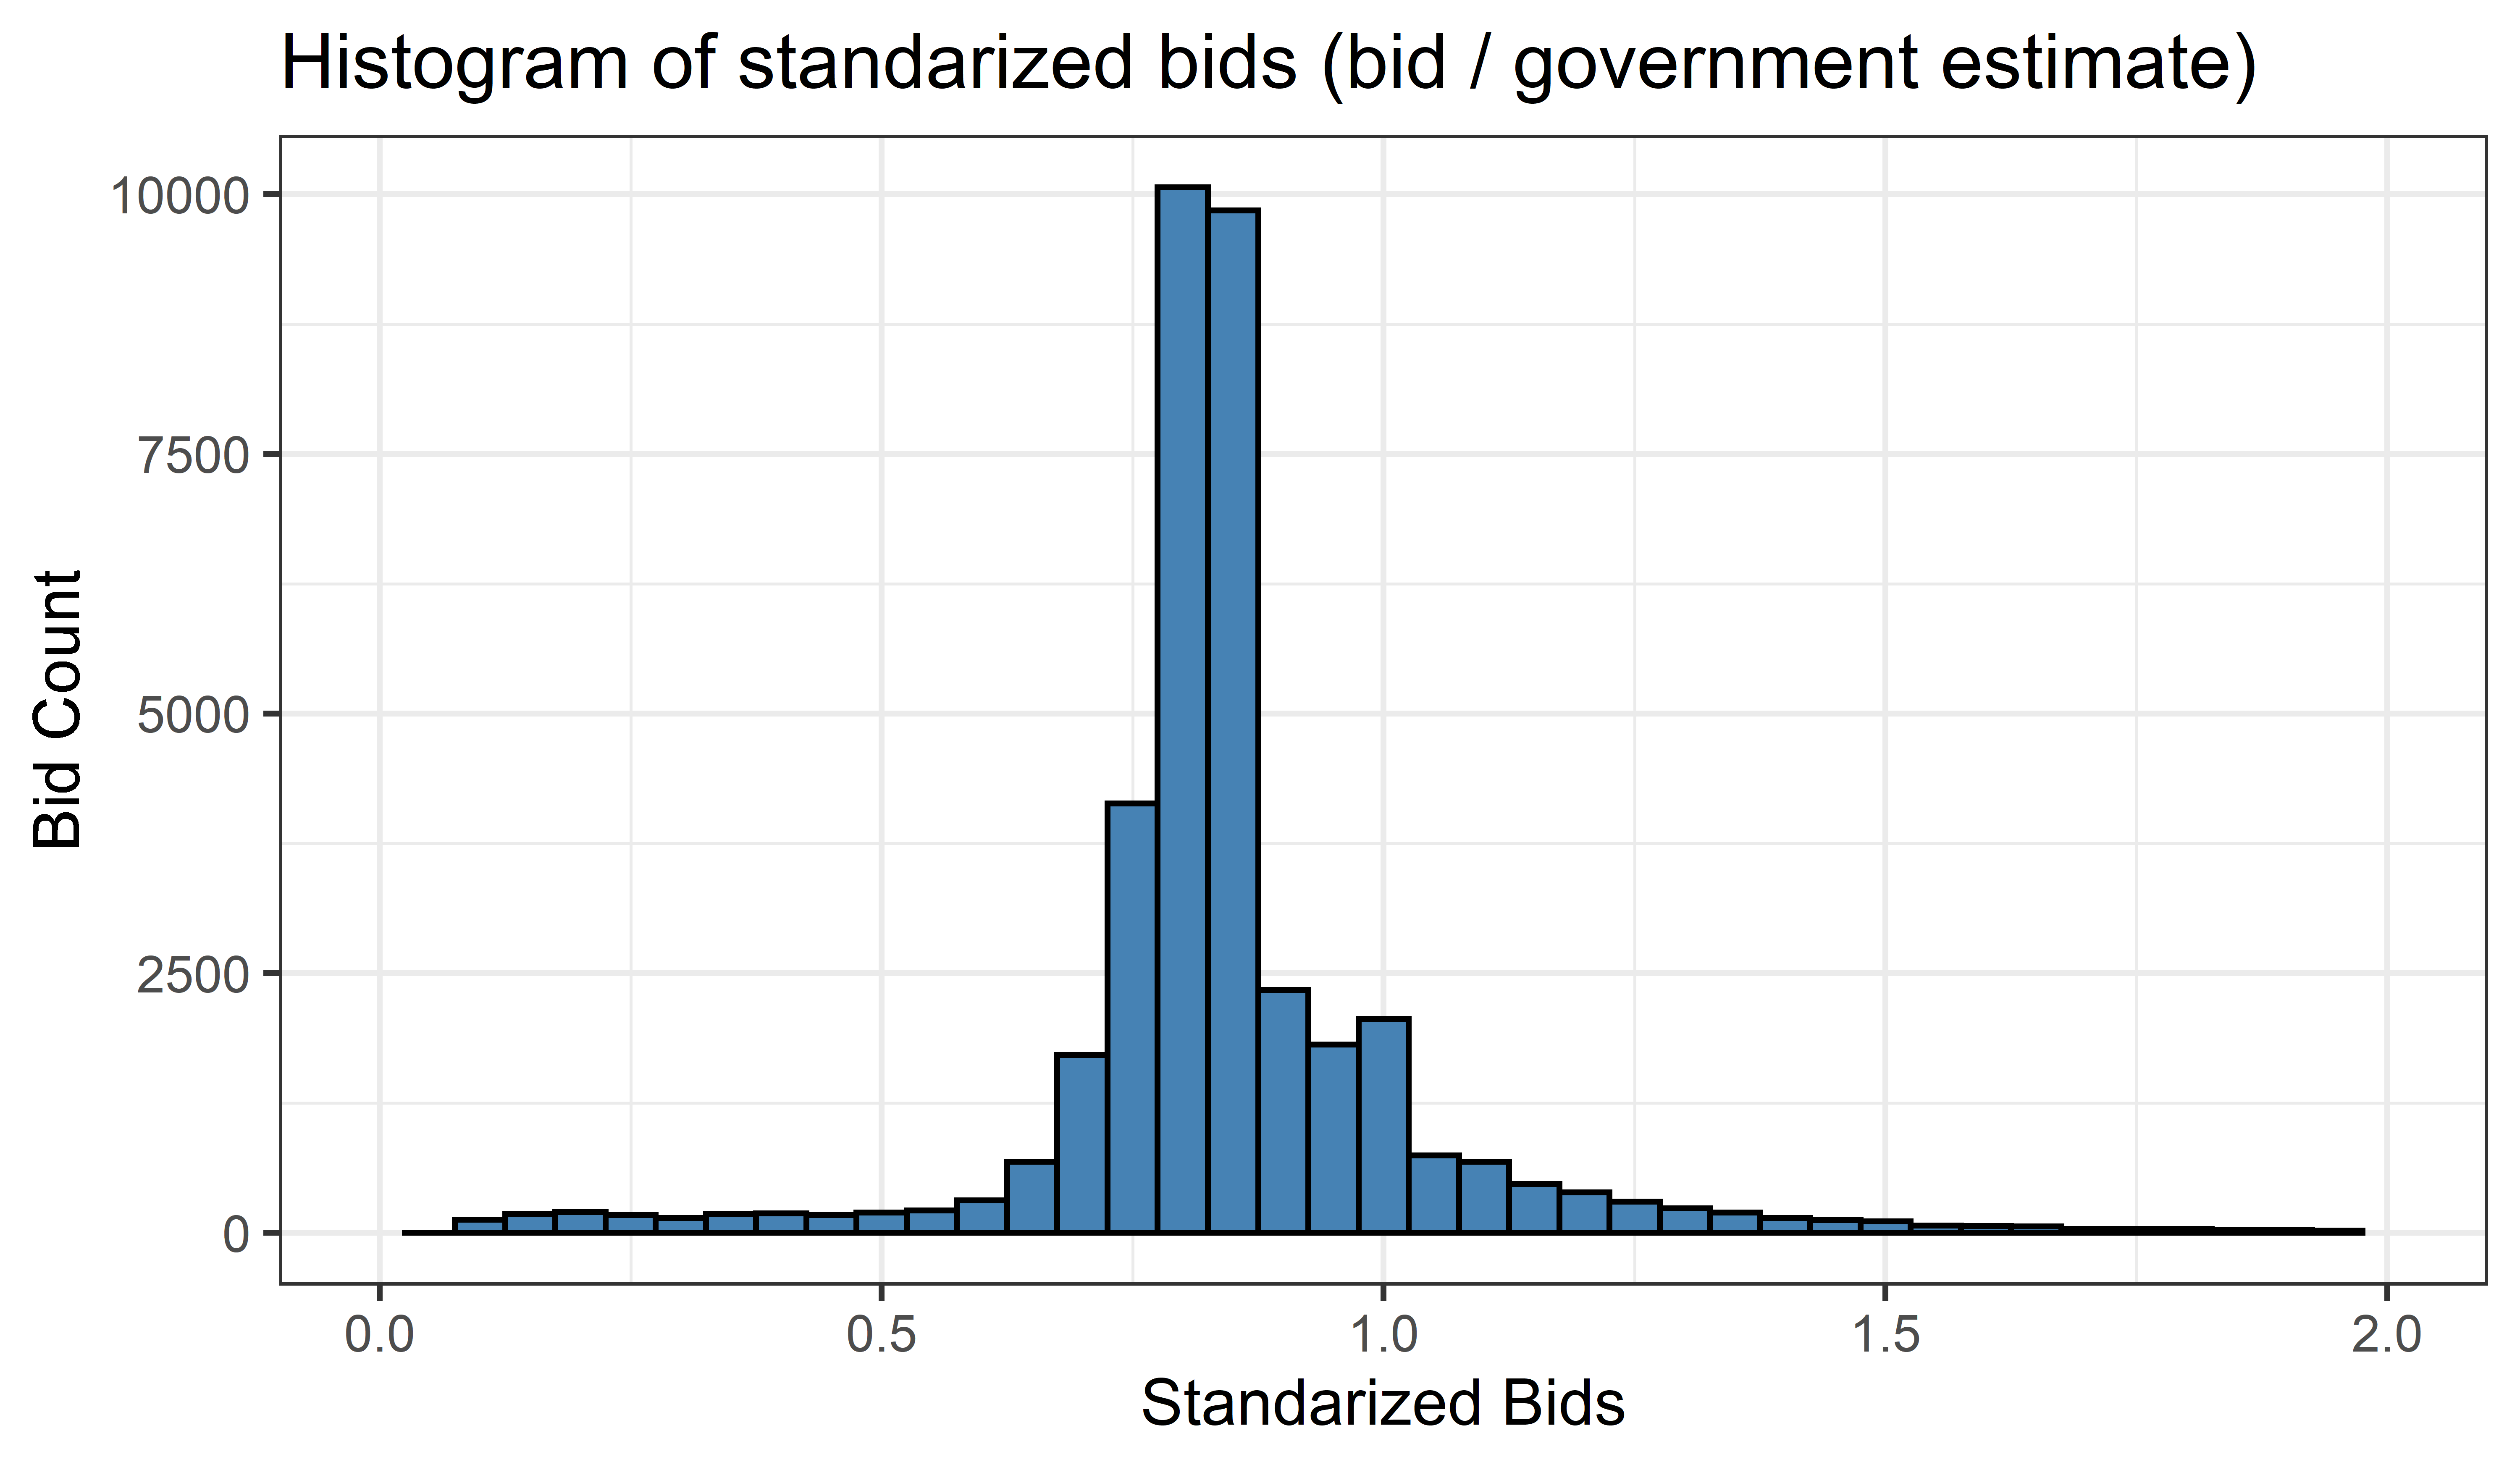
\includegraphics[scale=0.70]{plot_bids_standarized.png}
  \caption{Histogram of standarized bids}
  \label{fig:plot_bids_standarized}
\end{figure}

Table \ref{tab:table_bid_sample} shows descriptive statistics of the observations employed in the analysis sample for this section. Note that there are modifications with respect to Table \ref{tab:table_bid_sample}, given by the extra filtering steps employed for this analysis. \input{C:/repos/learn-doing/thesis/tables/table_bid_sample.txt}.

\subsection{Empirical Strategy}

Our empirical strategy relies on a regression of the form:
\begin{equation}
\label{eqn:olsbids}
BID_{ijt}=\alpha+ \beta EXP>0_{ijt}+X_j+FIRST_{ijt}+\varepsilon_{ijt}
\end{equation}
\begin{equation}
\label{eqn:olsbids2}
BID_{ijt}=\alpha+ \beta EXP_{ijt}+X_j+FIRST_{ijt}+\varepsilon_{ijt}
\end{equation}

Here, the outcome variable $BID_{ijt}$ is the standardized bid submitted by firm  $i$ at time $t$  to contract $j$. Our treatment variable is experience, either in binary form $EXP>0$ or linear form $EXP$. We compute experience by summing all contracts won up to $t$. Each bid in our main dataset (after the filtering steps detailed above) is an observation in the regression. We add controls $X_j$ corresponding to the region and year of the contract. Finally, we add an indicator variable $FIRST_{ij}$ which is 1 if firm $i$ is on its first year in the market when bidding for contract $j$, because from the theorical analysis and empirical literature we expect a positive effect due to "aggressiveness" of first entrants.

Similarly as before, we expect to have unobserved cost variables, specific to each firm, which might bias estimates upwards due to positive correlation with experience. We repeat the same strategy as before to produce consistent estimates, using closely won bids to produce random variation in total experience. The setting is an IV regression where we instrument $EXP_{it}$ with $EXPCLOSE_{it}$, the number of close wins by a firm up to time $t$. Wins are labeled as close wins if they fulfill the conditions established in the  previous chapter. For brevity, we only employ rank instruments in this section. %Table \ref{tab:closewins_bids} shows a comparison of bids identified as close wins (both by price and rank) against the rest of the sample.

Our consistency strategy relies in validity and relevance assumptions. The first one requires uncorrelatedness between close wins and cost measures. The second requires that our instrument does produce variation in the independent variable. We test this assumption by developing a regression of bids won on bids closely won (by price). The regression on wins on close wins by rank shows instead an F-statistic of 814 for the binary indicator and 631 for linear experience. Finally, to interpret our indicator estimate as the LATE, we again require a monotonicity condition, which is satisfied by construction.
%Based on these results, we abandon our first instrument (close wins by price) and we only keep the second alternative (close wins by rank). Note that contrary to the previous chapter we use outcomes at the individual bid level, which could explain this result.
%\input{C:/repos/learn-doing/thesis/tables/table_closewins_bids.txt}
\subsection{Results}
We show graphical results in Figure \ref{fig:plotbids_panel}. Panel A shows standardized bids against experience, employing all bids and firms in the sample. It can be seen that the average bid for firms without experience (0.89) is higher than the average of firms with any amount of positive experience. Panel B shows only firms with either one close win (by rank) or zero wins. Notably, firms with one close win (and no regular wins) submit bids that are on average almost 9 percentage points lower that those firms without experience. This equals around 40\%  of the standard deviation of standardized bids (0.23).

\begin{figure}[H]
  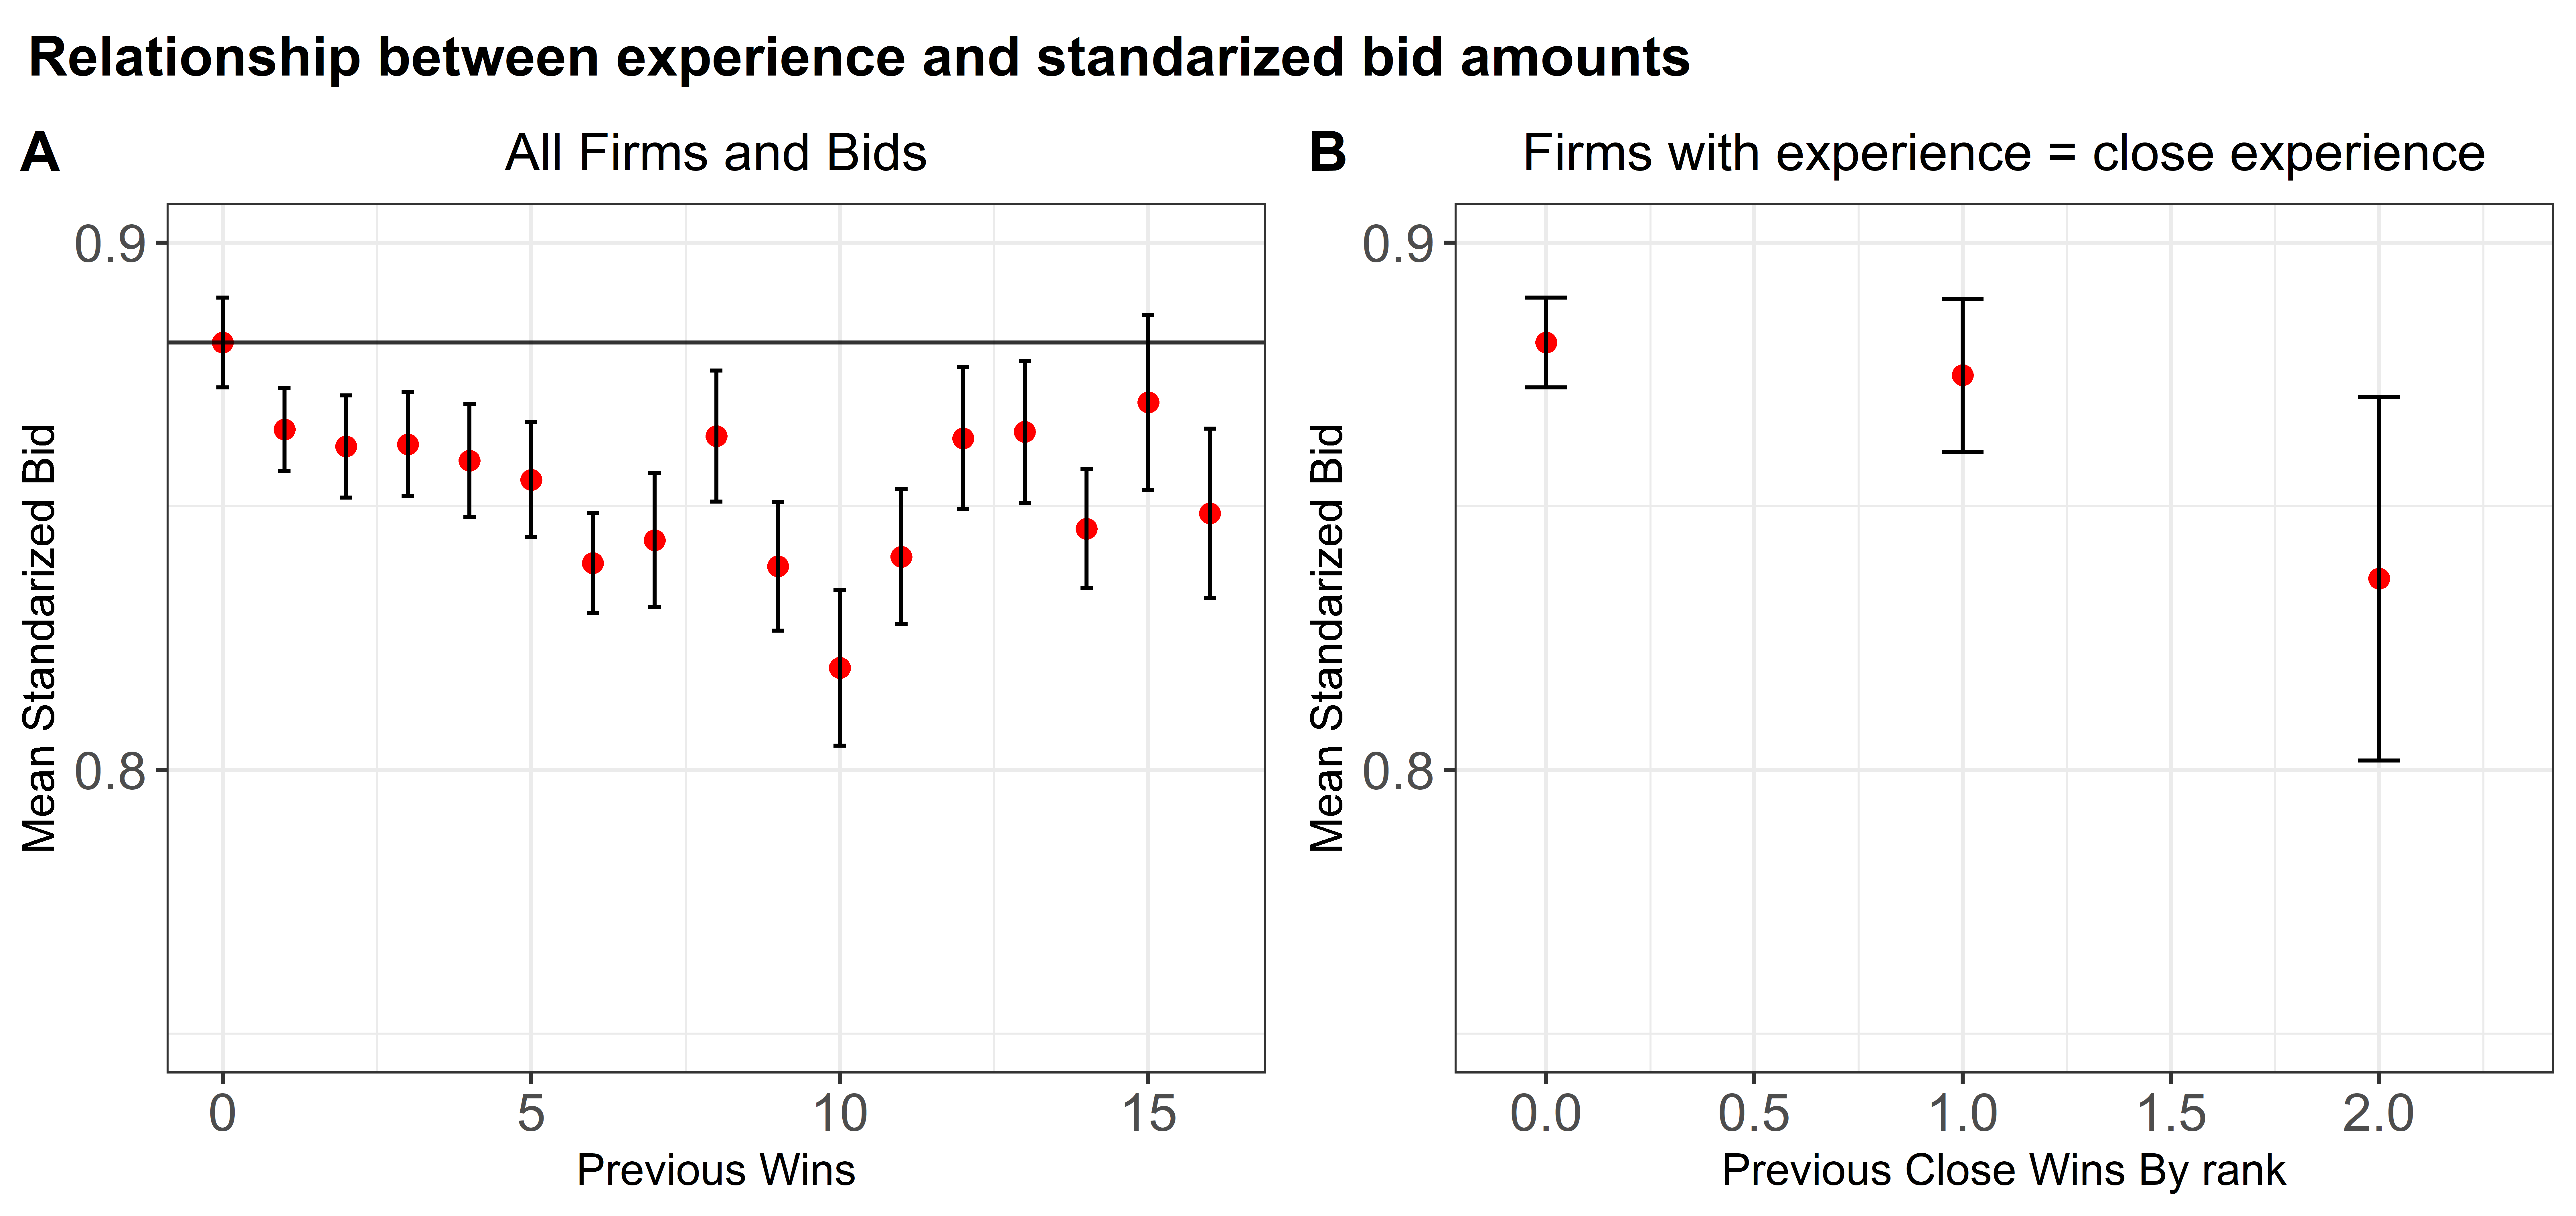
\includegraphics[scale=0.65]{plotbids_panel.png}
  \caption{Relationship between experience and standardized bid amounts}
  \label{fig:plotbids_panel}
\end{figure}

We perform four regressions between experience and standardized bids. The first two are the OLS and IV results employing binary experience as treatment; while the third and fourth are the OLS and IV regressions employing total experience as treatment. Table \ref{tab:table_bids_1} presents our main results. The OLS estimates of the effect of having experience on bid amounts is around -0.03 for OLS estimates and -0.024 for IV estimates. Although this is only around 15\% of the standard deviation of the standardized bid, given that the average difference between the lowest and second lowest bid is around eight percentage points, the effect is relevant to auction outcomes.

The linear OLS estimate is very small and the IV result is not significant. For this specifications, we obtain higher standard errors that prevents us from obtaining a precise estimates of the level of the treatment effects. We advance a possible explanation of this result based on our empirical strategy. Since now we examined experience fully cumulatively, after 10 years we might have extremely highly experienced firms which means higher variance in the independent variable, while the links between i) experience and bids and ii) close and regular wins decrease in strength. Among highly experienced firms, it is probable that the effect of experience is not relevant anymore and close wins do not have as a close relation with outcomes.

\input{C:/repos/learn-doing/thesis/tables/table_bids_results_1.txt}

Notwithstanding higher standard errors, our main hypothesis of interest, which was that experience produces cost advantages among treated firms, seems to be substantiated by the results. Although we cannot speak with certainty about the levels of the effect, we can conclude that experience does allow firms to submit lower bids as a source of competitive advantage. Results show treatment effects implying bids at least two percentage points higher on average for firms without experience compared with firms with strictly positive experience.

%%%%%%%%%%%%%%%%%%%%%%%%%%%%%%%%%%%%%%%%%%%%%%%%%%%%%%%%%

\section{Quality and Experience}
\label{section:qualityexp}
In order to test hypothesis number two, in this section we study if experience treatments causes firms to submit higher quality proposals. We proceed by analyzing whether experienced firms have higher proposal acceptance rates in the first stage of the awarding process, in which government units in charge of the auction discard proposals that do not fulfill basic formal requirements and/or technical specifications.

Recall that, for each auction, firm proposals are analyzed in two steps. The first step examines mostly if the proposals fulfill formal requirements. Formal requirements include the inclusion of required legal documents, submitting each of the technical documents asked for in the bidding documents, etc. In essence, the first stage verifies that all proposals can be evaluated in equal terms and that the minimum legal requirements are fulfilled. Clearly, whether a proposal was accepted is a measure of its quality, albeit an imperfect one. Although it leaves out a significant part of the variation that would be expected in proposal's qualities, it is nonetheless an interesting measure of quality because formal acceptance is a necessary condition to win a project.

Note that quality is explicitly evaluated in many contracts by including an item in the awarding criteria labeled as "technical specifications" or just "quality of the proposal". Employing string pattern matching, it is estimated that around 30\% of contracts include some measure of technical evaluation in the awarding criteria.  Ideally, we would test the hypothesis that experience improves the quality of a firm's proposals by employing the score that each firm obtained in the technical or quality item of the evaluation criteria of the project. However, since our data has not this item available by firm, we employ this alternative strategy.

Our research design, detailed below, tests whether experienced firms have a higher formal acceptance rate than unexperienced firms at the first stage of the awarding process.

\subsection{Data}
We employ our bid dataset similarly as in the previous chapter. We create time slices exactly as detailed in Section \ref{section:main_empirical} so we do not repeat the explanation of the full process.  Each observation consists in the outcomes of a firm in period 2 of slice $t$ and experience acquired during period 1 of the same slice $t$.

 Due to possible self-selection effects for firms with experience, we still filter out contracts which include experience in the awarding factor for outcome computation. We again filter the first year of the data in our analysis sample to prevent confounding effects.

To compute outcomes an indicator variable $INDACC_{ijt}$ is employed, which is 1 if the proposal submitted by firm $i$ at time $t$ for contract $j$ is accepted or not. The aggregated outcome is the mean of this indicator variable across the proposals submitted during the outcome period.

We show a histogram of the acceptance rates in Figure \ref{fig:plot_acceptance_rates}. We can already see that the fraction of firms getting all proposals rejected decreases if we consider firms with more than one proposal, which could be caused by the effect of learning about the formal revision stage after the first few bidding processes.

\begin{figure}
  
\includegraphics[scale=0.50]{plot_acceptance_rates.png}
  \caption{Histograms of proposal acceptance rate by firms in the dataset}
  \label{fig:plot_acceptance_rates}
\end{figure}

\subsection{Empirical Strategy}
We test whether experience leads to a higher rate of formal proposal acceptance employing the following regression:

\begin{equation}
\label{eqn:olsspec}
ACCRATE_{it}=\alpha+ \beta EXP_{it-1}+T_t+\varepsilon_{it}
\end{equation}

Here, $ACCRATE_{it2}$ is the share of proposals accepted out of proposals submitted in period 2 of slice $t$, $EXP_{it1} $ is the measure of experience employed for firm $i$ in slice $t$ (gained in period 1), and $T_t$ are period fixed effects. We employ indexes 1 and 2 to make explicit that each slice has two periods: one of experience computation and one of outcome computation, and every slice is indexed by $t$, which is date in between the two periods.

To be more explicit, let $C_{itk}$ be the set of contracts where firm $i$ submitted a proposal at period $k$ of slice $t$. Then, the outcome variable $ACCRATE_{it2}$ can also be written as:
$$  ACCRATE_{it2}=\dfrac{\sum_{j\in C_{it2}}INDACC_{it2}}{|C_{it2}|}$$

%Here, is and indicator variable that equals 1 if the firms' $i$ proposal for contract $j$ at time $t$ was accepted and zero if it was not. $EXP$ is our treatment variable, both in binary and linear functional forms. $X_{j}$ is a set of contract-specific controls, which include year, region, and the government body in charge of the auction. We include the controls for the possibility that government units in different  geographical regions have different levels of stringency when evaluating proposals for similar projects.

Additionally to unobserved cost advantages that could be endogenous to experience, we expect different levels of baseline levels of proposal-making abilities among firms, so we repeat our instrumentation of experience with close wins the same as the previous chapter and section. Since we apply the same sample procedure as in the previous chapter, the same discussion and results about validity and rank applies.

We perform six regressions between proposal acceptance rates and experience. The first three are the OLS and IV results employing our binary treatment; and the third to sixth employ a linear experience treatment. We employed our first alternative to compute experience, i.e. we employ two year periods to compute experience and subsequent two year periods to compute outcomes.

\subsection{Results}
Figure \ref{fig:plot_acceptance_results} displays graphic results. Panel A displays a clear discontinuity between the mean of the acceptance indicator variable for proposals sent by firms without experience and firms with any amount of positive experience. The mean acceptance rate for firms with no experience is .73, whereas it is equal or above .80 for proposals belonging to firms with positive experience.

To be more stringent with the sample, panel B displays the same analysis but here we leave out all firms except those which have only one previous proposal (won or lost), so they are new entrants to the market which may have won or lost their first contract (we analyze their next submitted proposal).  Notably, mean acceptance rates increase from .75 ($N=4,374$) for firms which lost their first auction to .87 ($N=990$) for firms which won their first auction.

Furthermore, we find that, for observations in the first quintile of acceptance rate, 40\% of them correspond to firms with strictly positive experience. On the other side, only 20\% of the observations in the first quintile of acceptance come from firms with no experience (at the point of observation, since a firm can be in both quintiles at different points in time).

Panels C and D show the mean acceptance rate against close experience as per the instrument level. We consider only firms having equal experience to close experience. In Panel C, the instrument is close experience by price and in D the instrument is close experience by rank. In both panels, we see an increase in the mean acceptance rate, although the sample is so reduced in panel C that we obtain very big standard errors.

Our regression results are shown in Table \ref{tab:table_acceptance_1}. The first three panels show the results for binary experience as treatment and the last three the treatment is total experience. We find positive and significant treatment effects of experience on outcomes: having positive experience results in almost 10 percentage points higher mean acceptance rates in future proposals (next two years). This means that having experience increases acceptance rates in around a third of a standard deviation of the outcome variable (.32). The IV results are close to OLS estimates, however, the standard errors are higher.

Regarding the treatment effect per unit of experience, we find that each new contract performed increases mean acceptance rates by around 1.2 percentage points. Again, the IV results are almost the same as the OLS results for the two alternative instruments.
 \clearpage
\begin{figure}
\centering
  \includegraphics[scale=0.65]{plot_acceptance_results.png}
  \caption{Acceptance rate for proposals sent by firms to auctions for public construction project.}
  \label{fig:plot_acceptance_results}
\end{figure}

\input{C:/repos/learn-doing/thesis/tables/table_acceptance_1.txt}
